\documentclass{report}
\usepackage{draftwatermark}
\SetWatermarkText{ }
\SetWatermarkScale{1}
\title{Radio Collar Tracker Flight Operations Manual}
\author{Eric Lo, Project Manager\\Nathan Hui, Project Lead\\Engineers for Exploration, UC San Diego}
\date{\today\\v2.0}
\usepackage{fullpage}
\usepackage{mdframed}
\usepackage{bookmark}
\usepackage{pdflscape}
\usepackage{multicol}
\usepackage{lmodern}

% Glossaries Definition
\usepackage[toc,nonumberlist]{glossaries}
\makeglossaries
\newacronym{COG}{COG}{Center Of Gravity}
\newacronym{UAS}{UAS}{Unmanned Aerial System}
\newacronym{GCS}{GCS}{Ground Control System}
\newacronym{PIC}{PIC}{Pilot In Command}
\newglossaryentry{multirotor}{
	name=multirotor,
	description={is an unmanned aircraft with multiple propellers for lift},
	plural=multirotors
}
\newglossaryentry{quadcopter}{
	name=quadcopter,
	description={is a multirotor with 4 propellers},
	plural=quadcopters
}
\newglossaryentry{LiPo}{
	name=LiPo,
	description={is a battery using a lithium polymer chemistry},
	plural=LiPos
}
\newglossaryentry{sdr_gls}{
	name={Software Defined Radio},
	description={is a radio that uses software instead of hardware to process and interpret the signal},
	plural={Software Defined Radios}
}
\newacronym[see={[Glossary:]{sdr_gls}}]{SDR}{SDR}{Software Defined Radio\glsadd{sdr_gls}}
\newacronym{RTL}{RTL}{Return To Launch}
\newacronym{AO}{AO}{Autopilot Operator}
\newacronym{VO}{VO}{Visual Observer}
\newacronym{COTS}{COTS}{Commercial Off-The-Shelf}
\newacronym{LOS}{LOS}{Line-Of-Sight}

\usepackage{hyperref}
\hypersetup{
    colorlinks,
    citecolor=black,
    filecolor=black,
    linkcolor=black,
    urlcolor=blue
}

\renewcommand*{\chapterautorefname}{Chapter}

\begin{document}
\maketitle
\tableofcontents
\chapter{Manual Objective}
	This manual is intended for the end user of the Radio Collar Tracker system.  It is written with the expectation that the end user has some experience flying \glspl{multirotor} in semi-autonomous or autonomous modes.  This manual should not be regarded as standalone training manual for flight operations, rather, it should part of hands-on training on how to operate this system safely.  This manual contains procedures on how to safely operate this system, as well as information on how to maintain and repair the system.
\chapter{System Overview}
	\section{Mission Profile}
		This system is designed to conduct aerial surveys for the purpose of tracking and localizing wildlife collars used for biological and ecological research.  We approach this problem by flying a radio across the search area, recording the signal strength for any pings from any collars we can detect.  We can then determine the location of a collar by correlating the signal strength and the locations where we detected that particular signal strength.

		\subsection{Phases of Flight}
			The overall flight can be broken up into multiple phases of flight: pre-takeoff, takeoff, climb, survey, approach, landing, and post-landing.

			The pre-takeoff phase of flight involves configuring and setting up the system for the intended survey.  This includes completing all relevant checks, flight planning, and maintenance.

			The takeoff phase of flight involves getting the system into the air in a safe and controlled manner.  This includes the initial climb to clear any obstacles in the takeoff zone.  This may be conducted manually or via automated mission command.

			The climb phase of flight involves getting the system to the survey objective area.  This may be conducted manually or via automated mission command.

			The survey phase of flight is the largest chunk of the flight time, and is usually conducted under complete autopilot control.  This is the phase of flight where the system is actively looking for collars.

			The approach phase of flight involves getting the system from survey altitude to the landing altitude.  This may be conducted manually or via automated mission command.

			The landing phase of flight involves getting the system out of the air and on the ground in a safe and controlled manner.  This includes the final descent to clear any obstacles in the landing zone.  This may be conducted manually or via automated mission command.

			The post-landing phase of flight involves securing the system, and safely shutting down all equipment.

			Many, if not all, of these phases of flight may be programmed as part of the automated mission.  This system can be automated to the point where the autopilot is responsible for takeoff, climb, survey, approach, and landing.
	\section{Aircraft}
		\subsection{Aircraft Summary}
			The airframe used in this \gls{UAS} is a 3DR Solo, which is a \gls{COTS} \gls{quadcopter}.  We have then added an independent payload that does not interface with the aircraft control system.
		\subsection{Aircraft Specifications}
			See Section 11.1 in the 3DR Solo User Manual.
		\subsection{Transmitter Layout}
			See Sections 1.3 and 5.6 in the 3DR Solo User Manual.
		\subsection{Aircraft Layout}
			See Section 1.2 in the 3DR Solo User Manual
	\section{Payload}
		\subsection{Payload Summary}
			The payload for this \gls{UAS} is a computerized radio recorder.  We have elected to use a software defined radio as our radio front end, as this allows us to rapidly reconfigure the payload for any range of frequencies.  This is connected to an Intel Joule, which handles all of the data collection, including collecting position data from the autopilot system.  Recorded data is organized into runs, which are stored on an SD card.
		\subsection{Payload Specifications}
			\begin{itemize}
				\item Computer\hfill Intel Joule
				\item Radio \hfill USRP B200-mini(-i)
				\item Weight \hfill 125 g
			\end{itemize}
	\section{Ground Control System}
		The \gls{GCS} for this \gls{UAS} consists of a laptop running a Windows OS and the open source flight management software, MissionPlanner.  This connects to the aircraft over the SoloLink WiFi network, permitting 2-way digital communications between the \gls{UAS} and the \gls{GCS}.  From the \gls{GCS}, we are able to plan, upload, and control all missions, as well as provide the pilot with flight and diagnostic information.
		
		See \autoref{chap:FMS}.
	\section{Crew Roles}
		\subsection{Pilot In Command}
			The \gls{PIC} is responsible for the safe operation of the aircraft.  He or she is responsible for takeoff, transition to survey, return, and landing, as well as for the general pacing of the mission.
		\subsection{Autopilot Operator}
			The \gls{AO} is responsible for monitoring the flight management software and survey progress.  He or she must plan and upload the mission plan to the aircraft, confirm clearance for switching to autonomous flight modes, and monitor the \gls{UAS} as it completes the mission.  The \gls{PIC} may also take on these duties so long as doing so does not jeopardize the safety of bystanders or the aircraft.
		\subsection{Visual Observer}
			The \gls{VO} is responsible for spotting the aircraft as it flies near flight operations area boundaries.  The \gls{VO} should have some form of communications link to the PIC, and should notify the PIC if the \gls{UAS} violates any area boundaries or comes near an obstacle.  Additionally, the \gls{VO} is responsible for recovering a downed \gls{UAS} to avoid disruption of any other activities in the area, and to maintain safety within the flight operations area boundaries.

			Having a \gls{VO} does not relieve the \gls{PIC} of the responsibility of maintaining \gls{LOS} to the \gls{UAS}.
\chapter{Checklists and Flight Procedures}
	The \gls{PIC} must use the below checklists and procedures when operating the system to ensure safe and proper operation of the system.  Failure to complete all items in either checklists or procedures may result in system misconfiguration or system failure.  The \gls{PIC} is responsible for the operation of the aircraft in accordance with all relevant rules and procedures, except that the \gls{PIC} may deviate from these rules where such deviation is necessary in the interests of safety.
	\section{Battery Cold Swap Procedure}
		See Section 2.3.2 in the 3DR Solo User Manual
	\section{Preflight Inspection}
		The \gls{PIC} must complete this checklist prior to each flight, to ensure that the aircraft is safe to operate and configured correctly.  This is referenced as ``Preflight Aircraft'' on the Reference Card.
		\begin{enumerate}
			\item Aircraft Docs \hrulefill Check present.
			\item Balance \hrulefill Check that \gls{COG} is centered.
			\item SOLO BATTERY POWER SWITCH \hrulefill Set to OFF position.
			\item SOLO CONTROLLER POWER SWITCH \hrulefill Set to OFF position.
			\item SOLO BATTERY LEVEL \hrulefill Check $>$ 90\%
			\item SOLO CONTROLLER BATTERY LEVEL \hrulefill Check $>$ 25\%
			\item SDR MOUNT \hrulefill Secure in place.
			\item SDR USB CONNECTOR \hrulefill Secure in place.
			\item SDR SMA CONNECTOR \hrulefill Secure in place.
			\item SDR ANTENNA \hrulefill Secure in place.
			\item GPS \hrulefill Secure in place.
			\item GPS USB CONNECTOR \hrulefill Secure in place.
			\item PAYLOAD POWER CONNECTOR \hrulefill Secure in place.
			\item PAYLOAD USB CONNECTOR A \hrulefill Secure in place.
			\item PAYLOAD USB CONNECTOR B \hrulefill Secure in place.
			\item PAYLOAD MOUNT \hrulefill Secure in place.
			\item PAYLOAD WIFI ANTENNA \hrulefill Secure in place.
			\item Propellers \hrulefill Check that propellers are tightened.
			\item Landing Gear \hrulefill Check that landing gear are securely attached.
		\end{enumerate}
	\section{Pre Power On Check}
		\begin{enumerate}
			\item Preflight Inspection Checklist \hrulefill Complete
			\item PAYLOAD SWITCH \hrulefill Set to OFF position.
		\end{enumerate}
	\section{Power On Procedure}
		This procedure is to be completed as part of the pre-takeoff phase of flight, prior to the takeoff phase of flight.  At the end of this procedure, the aircraft and payload will have been powered up and in an idle and safe state.
		\begin{enumerate}
			\item SOLO BATTERY POWER \hrulefill Hold for 5 seconds.
			\item SOLO LEDs \hrulefill Check White in front, Red in rear.
			\item PAYLOAD STATUS LIGHT \hrulefill Check
			\item SOLO CONTROLLER POWER \hrulefill Hold for 5 seconds.
			\item SOLO CONTROLLER SCREEN \hrulefill Check for ``Hold FLY to start motors'' screen.
			\item GCS WIFI \hrulefill Check connected.
			\item GCS SOFTWARE \hrulefill Start MissionPlanner.
			\item MP LINK PORT \hrulefill Set to ``UDP''.
			\item MP LINK \hrulefill Connect.
			\item MP Local Port \hrulefill Set the local UDP port to 14550.
		\end{enumerate}
	\section{Pre-Takeoff Check}
		This check is to be completed just prior to entering the takeoff phase of flight.  At the end of this check, the aircraft will be in a state that is ready to fly.  All items within this checklist must pass to proceed to the Takeoff Procedure.
		\begin{enumerate}
			\item MP HUD \hrulefill Check that all warnings are cleared.
			\item MP PreFlight \hrulefill Check that all items are green.
			\item GPS STATUS \hrulefill Check that the GPS fix is a 3D fix.
			\item GPS SATS \hrulefill Check that at least 6 GPS satellites reported.
			\item GPS LOCATION \hrulefill Check that the GPS location is stable and reasonable.
			\item AIRCRAFT ORIENTATION \hrulefill Check that the aircraft reports a horizontal orientation.
			\item AIRSPACE \hrulefill Check that the local airspace is clear.
			\item TAKEOFF CLEARANCE \hrulefill Contact local ATC for takeoff clearance.
		\end{enumerate}
	\section{Payload Start Procedure}
		This procedure is to be completed during the pre-takeoff phase of flight, prior to the takeoff phase of flight.  The Aircraft and Payload Power On Procedure must be completed prior to executing this procedure.  At the end of this procedure, the payload will have been initiated and will be actively recording data.
		\begin{enumerate}
			\item PAYLOAD SWITCH \hrulefill Set to the ON position.
			\item PAYLOAD STATUS LIGHT \hrulefill Check for blinking.
		\end{enumerate}
	\section{Takeoff Procedure}
		This procedure is to be completed during the takeoff phase of flight, prior to the climb phase of flight.  The Pre-Takeoff Check must be completed prior to executing this procedure.  At the end of this procedure, the aircraft will be in a stable hover above the takeoff zone.
		\begin{enumerate}
			\item SOLO CONTROLLER FLY \hrulefill Hold until motor start.
			\item THROTTLE \hrulefill Set to 75\%.
		\end{enumerate}
	\section{Pre-Mission Start Check}
		This check is to be completed just prior to starting any automated mission irregardless of current phase of flight.  The aircraft must be on and stable prior to conducting this check.  At the end of this check, the aircraft will be in a state that is ready to start the mission.  All items within this checklist must pass to proceed to the Mission Start Procedure.
		\begin{enumerate}
			\item Power On \hrulefill Completed
			\item MISSION \hrulefill Uploaded and verified.
			\item WINDS \hrulefill Check $<$ 10 m/s.
		\end{enumerate}
	\section{Mission Start Procedure}
		This procedure is to be completed at the beginning of the mission phase of flight.  The Pre-Mission Start Check must be completed prior to executing this procedure.  At the end of this procedure, the aircraft will start the planned mission.
		\begin{enumerate}
			\item Pre-Mission Start \hrulefill Completed.
			\item LOCAL AIRSPACE \hrulefill Check that local airspace is clear.
			\item FLIGHT MODE \hrulefill Set to AUTO.
		\end{enumerate}
	\section{Mission End Procedure}
		This procedure may be completed at the end of the mission phase of flight.  This procedure may be completed at any point to regain control of the aircraft during a mission.  At the end of this procedure, the aircraft will be under the \gls{PIC}'s control.
		\begin{enumerate}
			\item FLIGHT MODE \hrulefill Set to LOITER.
		\end{enumerate}
	\section{Pre-Landing Checks}
		This check is to be complete prior to entering the approach phase of flight.  At the end of this check, the aircraft is cleared to begin the approach to the landing zone.
		\begin{enumerate}
			\item APPROACH \hrulefill Check that the APPROACH is clear of obstacles.
			\item TRAFFIC \hrulefill Check that no air traffic will interfere.
			\item FLIGHT MODE \hrulefill Set to LOITER.
		\end{enumerate}
	\section{Approach Procedure}
		This procedure is to be executed during the approach phase of flight.  At the end of this procedure, the aircraft will be ready to begin the landing procedure.
		\begin{enumerate}
			\item THROTTLE \hrulefill Reduce as needed.
			\item Descent Rate \hrulefill $<$ 2 m/s
		\end{enumerate}
	\section{Landing Procedure}
		This procedure is to be executed during the landing phase of flight.  At the end of this procedure, the aircraft will be on the ground and safed.
		\begin{enumerate}
			\item THROTTLE \hrulefill Reduce as needed.
			\item Descent Rate \hrulefill $<$ 2 m/s.
			\item THROTTLE \hrulefill 0\% upon ground contact.
		\end{enumerate}
	\section{Payload Stop Procedure}
		This procedure is to be executed during the post-landing phase of flight.  At the end of this procedure, the payload will be in an idle state, with the completed run saved.
		\begin{enumerate}
			\item PAYLOAD SWITCH \hrulefill Set to OFF position.
			\item PAYLOAD STATUS LIGHT \hrulefill solid.
			\item PAYLOAD STATUS LIGHT \hrulefill turns off within 1 minute.
			\item PAYLOAD READY LIGHT \hrulefill turns on after the PAYLOAD STATUS LIGHT turns off.
		\end{enumerate}
\chapter{Emergency Procedures}
	\section{Battery Fire on Ground}
		Battery fires are caused by extreme physical or electrical damage to the battery pack.  Battery fires may be preceded by significant warming and/or puffing of the battery pack.
		\begin{mdframed}[linecolor=red,linewidth=4pt]
			WARNING: \gls{LiPo} fires are chemical fires, and can release dangerous chemicals.  ABC fire extinguishers are NOT effective against the primary battery fire, but may prevent the fire from spreading.  If available, use a CO2, dry chemical, or foam extinguisher to contain the primary fire.  Do not use water to extinguish the primary fire, however, water may be used to cool a battery and fight secondary fires as appropriate.
		\end{mdframed}
		\begin{enumerate}
			\item If the battery has not caught fire yet, but is extremely warm, immediately unplug it from any devices and take the battery outside.  Place it away from flammable items and in a well ventilated area. Allow the battery to sit for at least 30 minutes.  If the battery has cooled down in 30 minutes, it will likely not catch fire, however, the battery must be disposed of properly.  If the battery is still hot, allow it to remain outside until it has cooled off.
			\item If the battery catches fire while connected to a charger, disconnect the charger from the wall, and, if safe to do so, carry the entire charging setup outside, away from flammable items and place in a well ventilated area. If not safe to do so, remove flammable items from the area and fight any secondary fires.  Do not fight the battery fire itself, as it is self-oxidizing.

			Even if the primary fire is out, if the pack is warm, additional cells may catch fire due to thermal loading.  The battery pack is not safe until the entire pack is cooled to room temperature.
			\item If the battery catches fire while connected to the aircraft, if safe to do so, remove the battery from the aircraft.  If unable to remove the battery, if safe to do so, flip the aircraft so that the battery is on top of the aircraft to reduce damage to the aircraft.  Carry the batteries and any attached items outside, away from flammable items and place in a well ventilated area.  If not safe to move the batteries, remove flammable items from the area and fight any secondary fires.  Do not fight the primary battery fire itself, as it is self-oxidizing.

			Even if the primary fire is out, if the pack is warm, additional cells may catch fire due to thermal loading.  The battery pack is not safe until the entire pack is cooled to room temperature.
		\end{enumerate}
	\section{Loss of Autopilot Datalink}
		If the autopilot operator reports loss of link to the \gls{UAS} (characterized by no data packets received for about 5 seconds), then the \gls{UAS} will automatically initiate an \gls{RTL}.  This will continue even if the aircraft datalink is recovered.  To recover, set the flight mode to LOITER.
\chapter{Maintenance}
	This section contains checklists and procedures to facilitate the maintenance and repair of the \gls{UAS}.  The \gls{UAS} must pass all items within the Delivery Check before being placed into service.  Failure of any one of these checks may result in system failure.
	\section{Charging Batteries}
		See Section 2.3.1 in the 3DR Solo User Manual.
	\section{Propellers}
		\subsection{Inspection}
		Nylon propellers should be replaced if they are damaged.  Visually inspect the propeller for abnormal tears or warping.

		\subsection{Removal}
		To remove the propeller, unscrew the propeller from the motor housing.  Silver-top propellers unscrew counterclockwise; black-top propellers unscrew clockwise.  Check the unlock icons on each propeller to see the correct directions for removing.

		\subsection{Installation}
		To install the propeller, screw the propeller onto the motor housing.  Silver-top propellers tighten clockwise; black-top propellers tighten counterclockwise.  Check the lock icons on each propeller to see the correct directions for tightening.
	
	\section{Payload Antenna}
		\subsection{Inspection}
			Ensure that the antenna is not bent or warped in any way.

		\subsection{Removal}
		To remove the payload antenna, first disconnect the payload antenna from the payload by unscrewing the SMA connector on the antenna.  Next, remove the antenna by removing the velcro straps holding the antenna to the copter.

		\subsection{Installation}
		To install the payload antenna, attach the antenna to the copter's left side using the provided velcro straps.  Ensure that the antenna is nestled in the corner made by the copter's arms and landing gear.  Next, connect the SMA connectors on the antenna and the payload.
	\section{Payload Hardware}
		\subsection{Inspection}

		\subsection{Removal}
		To remove the payload, first disconnect the payload power, autopilot telemetry cable, and payload antenna from the payload.  Next, remove the two screws holding the payload to the aircraft.

		\subsection{Installation}
		To install the payload, align the payload with the existing screw holes on the aircraft so that the user interface devices face the outside of the aircraft.  Install the two screws to secure the payload to the aircraft.  Connect the payload power, autopilot telemetry cable, and payload antenna to the payload.
\chapter{Flight Management Software}
	\label{chap:FMS}
	\section{Requirements}
		\begin{itemize}
			\item Minimum Operating System: Windows 7
			\item Known Good Mission Planner Versions: 1.3.37
		\end{itemize}
	\section{Installation}
		\begin{enumerate}
			\item Download the Mission Planner Installer from http://ardupilot.com
			\item Accept the default settings.
			\item Install the additional drivers when prompted to.
			\item Click finish.
		\end{enumerate}
	\section{Flight Planning}
		\begin{figure}[ht]
			\centering
			\caption{Mission Planner Flight Plan Screen}
			\includegraphics[width=\textwidth]{mp_flight_plan_screen.jpg}
			\label{fig:mp_flight_plan}
		\end{figure}
		\subsection{Setting the Home Position}
			The HOME position represents the takeoff/landing location for the copter.  Generally, if the \gls{GCS} is connected to the \gls{UAS}, then Mission Planner can automatically update the HOME position upon \gls{UAS} arm.  However, there are occasions when this is not possible.  There are two ways to set the HOME position.

			Option 1:
			\begin{enumerate}
				\item If the new HOME location is close to the old location, simply click and drag the HOME location balloon to the desired location.  The HOME location balloon is denoted by a bold ``H'' within the balloon, or with a small label.
			\end{enumerate}

			Option 2:
			\begin{enumerate}
				\item Click and drag the map view to the desired location.
				\item Click on the ``Lat'' field.
				\item Click ``OK''.
				\item Click on the desired HOME location.
			\end{enumerate}
		\subsection{Selecting a Search Area}
			\begin{enumerate}
				\item Right click to open the context menu.
				\item Under ``Draw Polygon'', select ``Add Polygon Point''.
				\item Click ``OK''.
				\item Drag the first point to the desired location.
				\item Click to set additional points.
			\end{enumerate}
		\subsection{Loading a Search Area}
			\begin{enumerate}
				\item Right click to open the context menu.
				\item Under ``Draw Polygon'', select ``Load Polygon''.
				\item Select the polygon file you wish to load.
			\end{enumerate}
		\subsection{Saving a Search Area}
			\begin{enumerate}
				\item Right click to open the context menu.
				\item Under ``Draw Polygon'', select ``Save Polygon''.
				\item Enter the filename and directory in which you would like to save the polygon file.
				\item Click ``Save''.
			\end{enumerate}
		\subsection{Plotting a Search Grid}
			\begin{enumerate}
				\item Set a search area.
				\item Right click to open the context menu.
				\item Under ``Auto WP'', select ``Survey (Grid)''.
				\item Check the ``Advanced Options'' checkbox under ``Display'' on the right-hand sidebar.
				\item Set the desired altitude and flight speed.
				\item Check the ``Add Takeoff and Land WP's'' and ``Use \gls{RTL}'' checkboxes.
				\item Open the ``Grid Options'' tab.
				\item Set the ``Distance between lines [m]'' to 30 meters.
				\item Check that the ``Flight Time (est)'' field on the bottom bar is less than 20 minutes.
				\item Click ``Accept''.
				\item Check that the waypoints have been properly set.
			\end{enumerate}
		\subsection{Saving a Mission}
			\begin{enumerate}
				\item Click the ``Save WPs'' button in the right-hand sidebar.
				\item Select the desired directory and filename and save.
			\end{enumerate}
		\subsection{Opening a Saved Mission}
			\begin{enumerate}
				\item Click the ``Load WPs'' button in the right-hand sidebar.
				\item Navigate to the desired waypoints file and click ``Open''.
				\item Click ``OK'' when prompted to replace the HOME location.
			\end{enumerate}
	\section{Uploading a Mission}
		\begin{enumerate}
			\item Load a mission into Mission Planner.
			\item Connect to the \gls{UAS} with MAVLINK.
			\item Click the ``Write WPs'' button on the right-hand sidebar.
			\item Click the ``Read WPs'' button on the right-hand sidebar.
			\item Click ``OK'' to the dialog prompting you to reset the HOME location.
			\item Verify that the waypoints now displayed are the desired mission waypoints.
		\end{enumerate}
	\section{Operating a Mission}
		\begin{figure}[ht]
			\centering
			\caption{Mission Planner Flight Data Screen}
			\includegraphics[width=\textwidth]{mp_hud_full.jpg}
			\label{fig:mp_flt_data}
		\end{figure}
		The primary responsibility of the \gls{AO} is to monitor the \gls{UAS} as it progresses through its programmed mission using the Flight Data Screen (\autoref{fig:mp_flt_data}).  During this time, the autopilot operator should be monitoring the vital signs from the \gls{UAS}, including ground speed, mission progress, altitude, attitude, stability, battery voltage, battery consumption, power draw, and navigation stability, among other things.  In most cases, monitoring the artificial horizon and flight map will suffice - check that the \gls{UAS} is tracking properly to the waypoints, and that the aircraft has a reasonable attitude for its current speed and heading.  In addition, the \gls{AO} can use the wireless telemetry connection readout as a gauge of the quality of the autopilot datalink.  Occasionally, check the battery voltage and consumption to ensure that the \gls{UAS} has enough power to complete the mission and return.
	\section{Connecting GCS MAVLINK}
		\begin{enumerate}
			\item Select UDP.  See \autoref{fig:MP_Connect}.
				\begin{figure}[ht]
					\centering
					\caption{Connection Settings for Mission Planner}
					\includegraphics{MisionPlanner_ConnectButton.png}
					\label{fig:MP_Connect}
				\end{figure}
			\item Click the ``CONNECT'' button.
			\item Set the local port to 14550 (default).
		\end{enumerate}	
		
\chapter{Operating the Ground Control Software}
	\begin{figure}[ht]
		\centering
		\caption{Interactive Drop-Downs for this Section}
		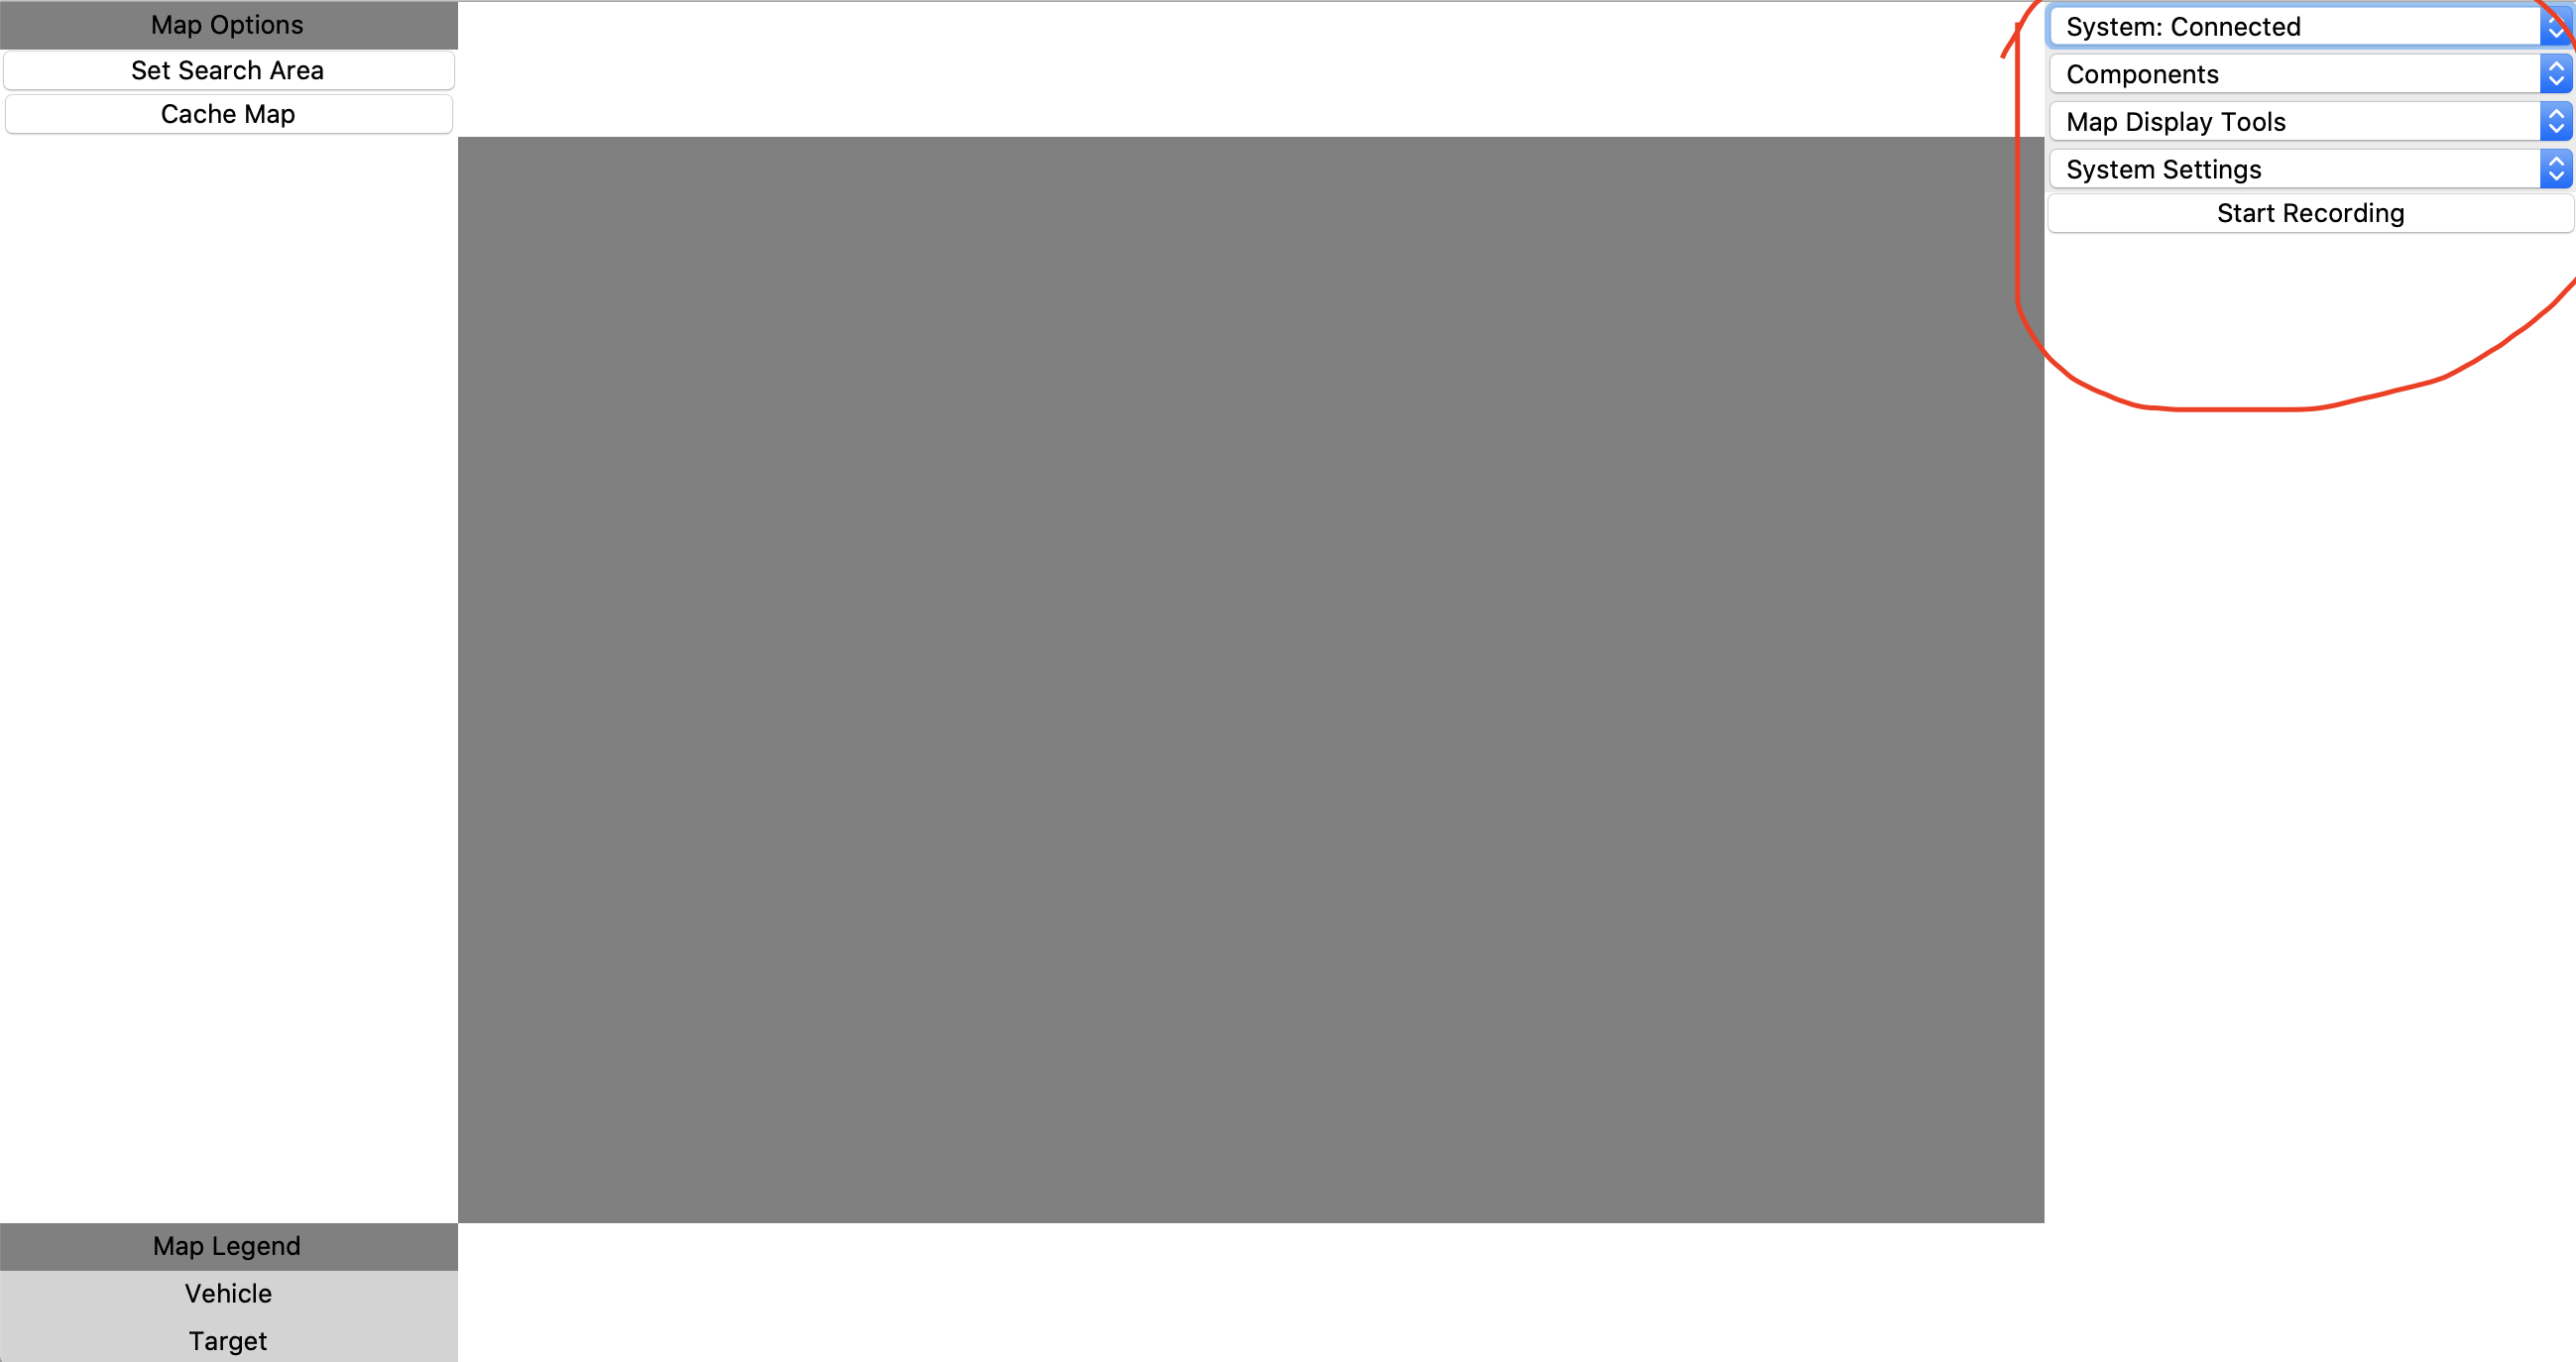
\includegraphics[width=\textwidth]{right_column_dropdowns.jpg}
		\label{fig:right_column_dd}
	\end{figure}
	\section{Connecting to the Payload}
		\begin{figure}[htb]
			\centering
			\caption{Connect Drop-Down}
			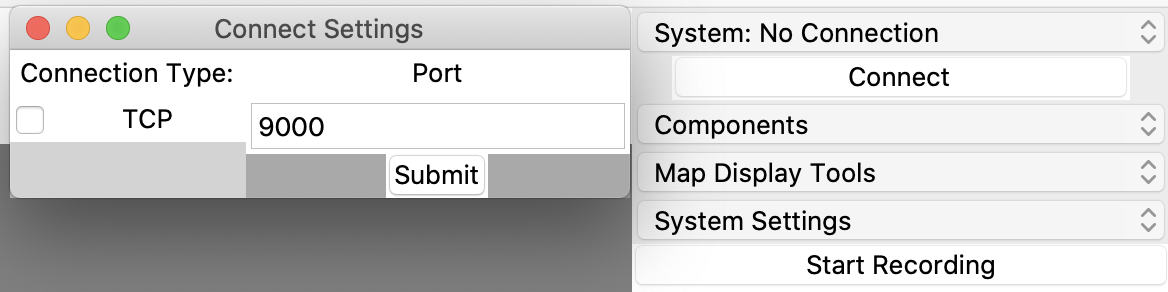
\includegraphics[scale=0.5]{connect_button.jpg}
			\label{fig:connect_button}
		\end{figure}
		\begin{enumerate}
			\item With the GCS open, locate the series of drop-downs in the right-most column of the user interface.
			\item Expand the drop-down titled ``System: Not Connected''.
			\item Click on the button labeled ``Connect''.
			\item In the resulting pop-up window (titled ``Connect Settings''), enter the port number the payload is located at. The default value should already be populated. 
			\item Highlight the TCP checkbox.
			\item Click on the button labeled ``Submit''.
			\item Confirm that the label on the same drop-down you expanded earlier now says ``System: Connected''.
		\end{enumerate}
	\section{Configuring the Payload}
		\subsection{Center Frequency, Sampling Frequency, and SDR Gain}
			\begin{figure}[htb]
				\centering
				\caption{System-Settings Drop-Down}
				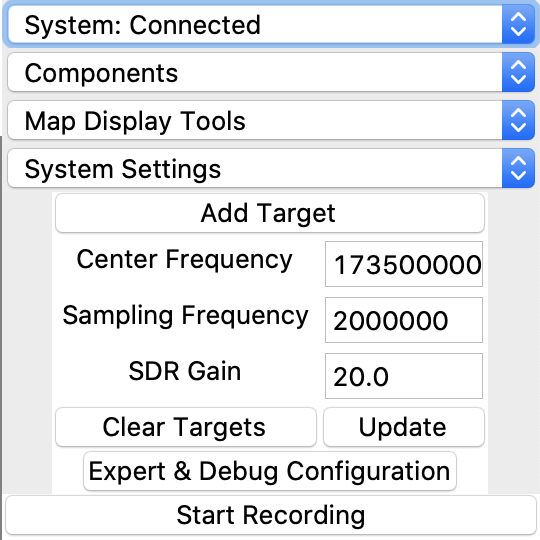
\includegraphics[scale=0.5]{system_settings_dd.jpg}
				\label{fig:system_settings_dd}
			\end{figure}
			\begin{enumerate}
				\item With the GCS open and connected to the payload, locate the series of drop-downs in the right-most column of the user interface.
				\item Expand the drop-down labeled ``System Settings''.
				\item The current values of the payload's center frequency, sampling frequency, and SDR gain are displayed. Edit any values to the desired values.
				\item Once finished editing, click on the button labeled ``Update''. 
				\item Confirm that the new values displayed in the drop-down are the new desired values.
			\end{enumerate}
			The following is a reference table explaining what each of these values signifies:
			\begin{table}[htb]
			\centering
			\caption{Payload system settings and their respective meanings.}
			\begin{tabular}{||c c c||}
			\hline
			Value & Meaning & Units\\ [0.5ex]
			\hline\hline
			Center Frequency & SDR center frequency. & Hz \\
			\hline
			Sampling Frequency & SDR sampling frequency. & Hz \\
			\hline
			SDR Gain & SDR gain. Higher values mean more attenuation. & dB \\ [1ex]
			\hline
			\end{tabular}
			\end{table}
		\subsection{Adding Target Frequencies}
			\begin{figure}[htb]
				\centering
				\caption{Add Target Frequency Button}
				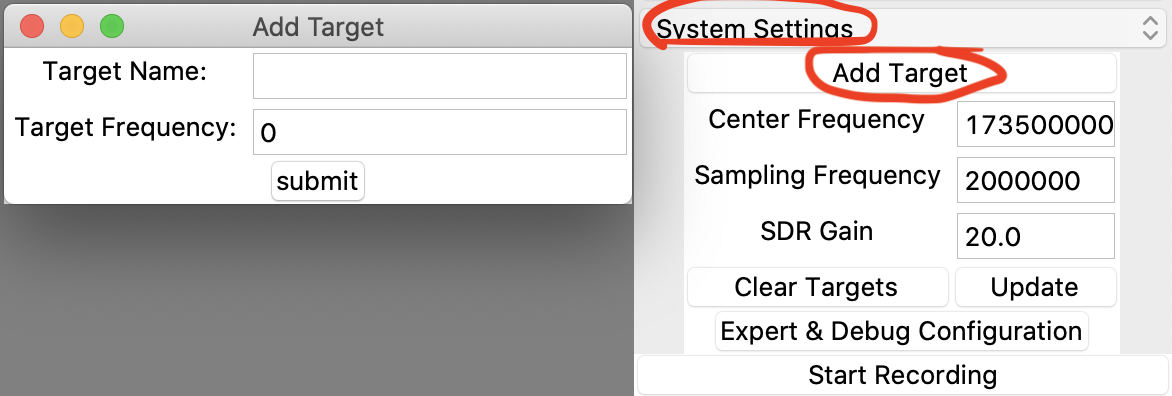
\includegraphics[scale=0.5]{add_target_btn.jpg}
				\label{fig:add_target_btn}
			\end{figure}
			\begin{enumerate}
				\item With the GCS open and connected to the payload, locate the series of drop-downs in the right-most column of the user interface.
				\item Expand the drop-down labeled ``System Settings''.
				\item Click on the button labeled ``Add Target'' located above the center frequency display.
				\item In the resulting pop-up window (titled ``Add Target''), enter the desired target name. If no target name is desired, leave the field blank and the target frequency will be assigned a generic name.
				\item Enter the value of the desired target frequency. The system will only accept a valid target frequency within the following range: [$F_c - F_s , F_c + F_s$] where $F_c$ is the center frequency and $F_s$ is the sampling frequency. 
				\item Click on the button labeled ``submit''. If an invalid frequency is entered, the system will prompt for a new target frequency value. Simply alter the value of the target frequency and click submit once again.
				\item Confirm that the new target frequency is displayed under the drop-down titled ``System Settings'' (it should be located under the SDR Gain field).
			\end{enumerate}
		\subsection{Deleting Target Frequencies}
			\begin{figure}[htb]
				\centering
				\caption{Delete Target Frequencies Button}
				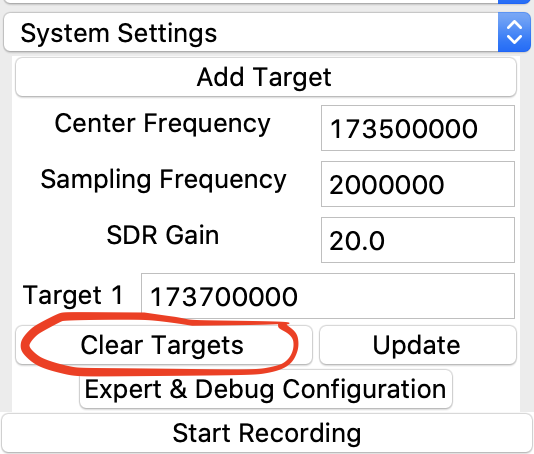
\includegraphics[scale=0.5]{delete_targets_btn.jpg}
				\label{fig:delete_targets_btn}
			\end{figure}
			\begin{enumerate}
				\item With the GCS open and connected to the payload, locate the series of drop-downs in the right-most column of the user interface.
				\item Expand the drop-down labeled ``System Settings''.
				\item Click on the button labeled ``Clear Targets''. This will clear all of the target frequencies entered.
				\item Confirm that no target frequencies remain in the drop-down. 
			\end{enumerate}
		\subsection{Expert and Debug Configuration}
			The Expert and Debug configuration panel is useful if there are desired values to be configured on the payload that are not addressed in the previous sections.
			\begin{figure}[htb]
				\centering
				\caption{Expert and Debug Configuration Button}
				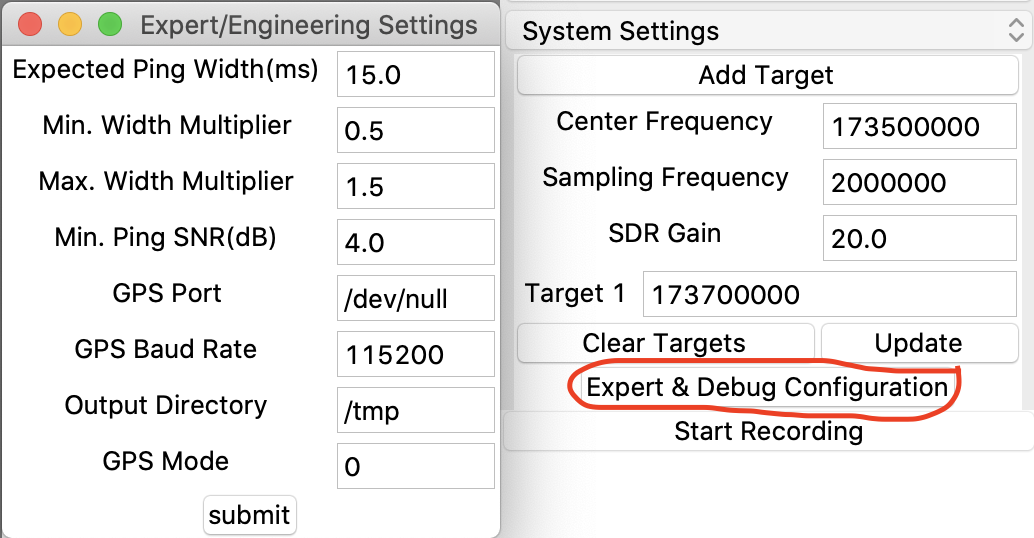
\includegraphics[scale=0.5]{expert_debug.jpg}
				\label{fig:expert_debug}
			\end{figure}
			\begin{enumerate}
				\item With the GCS open and connected to the payload, locate the series of drop-downs in the right-most column of the user interface.
				\item Expand the drop-down labeled ``System Settings''.
				\item Click on the button labeled ``Expert \& Debug Configuration''.
				\item In the resulting pop-up window (titled ``Expert/Engineering Settings''), enter the new desired values for the fields displayed.
				\item Once done editing, click on the button labeled ``submit''.
			\end{enumerate}
			The following is a reference table containing additional information about each of the Expert \& Debug settings.
			\begin{table}[htb]
			\centering
			\caption{Expert system settings and their respective meanings.}
			\begin{tabular}{||c c||}
			\hline
			Value & Meaning\\ [0.5ex]
			\hline\hline
			Expected Ping Width & Normal ping width (ms). \\
			\hline
			Min. Width Multiplier & Minimum acceptable ping width multiplier. \\
			\hline
			Max. Width Multiplier & Maximum acceptable ping width multiplier.\\
			\hline
			Min. Ping SNR & Minimum acceptable ping signal to noise ratio (dB). \\
			\hline
			GPS Port & Path to GPS serial port.\\
			\hline
			GPS Baud Rate & GPS serial port baud rate.\\
			\hline
			Output Directory & Location where are SDR record info is outputted.\\
			\hline
			GPS Mode & GPS test mode.\\ [1ex]
			\hline
			\end{tabular}
			\end{table}
	\section{Checking on the Payload Status}
		\begin{figure}[htb]
			\centering
			\caption{Component Status Drop-Down}
			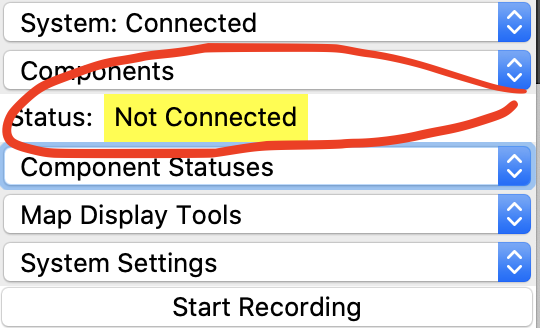
\includegraphics[scale=0.5]{component_status_dd.jpg}
			\label{fig:component_status_dd}
		\end{figure}
		The payload has four possible states: 
		\begin{table}[htb]
			\centering
			\caption{System statuses and their respective meanings.}
			\begin{tabular}{||c c||}
			\hline
			State & Meaning\\ [0.5ex]
			\hline\hline
			Not Connected & At least one of the components of the payload is not ready to record. \\
			\hline
			Idle & All components of the payload are ready. \\
			\hline
			Running & The payload is recording. \\
			\hline
			Stopping & The payload is in the process of ending the recording. \\
			\hline
			Failed & At least one of the components of the payload has failed. \\ [1ex]
			\hline
			\end{tabular}
		\end{table}
		To check on the status of the payload:
		\begin{enumerate}
			\item With the GCS open and connected to the payload, locate the series of drop-downs in the right-most column of the user interface.
			\item Expand the drop-down labeled "Components".
			\item The entry next to "Status" is the current status of the payload.
			\item If additional information about the status of individual components within the payload is desired, refer to the following subsection.
		\end{enumerate}
		\section{Checking the Status of Individual Components Within Payload}
			\begin{figure}[htb]
				\centering
				\caption{Individual Component Status Drop-Down}
				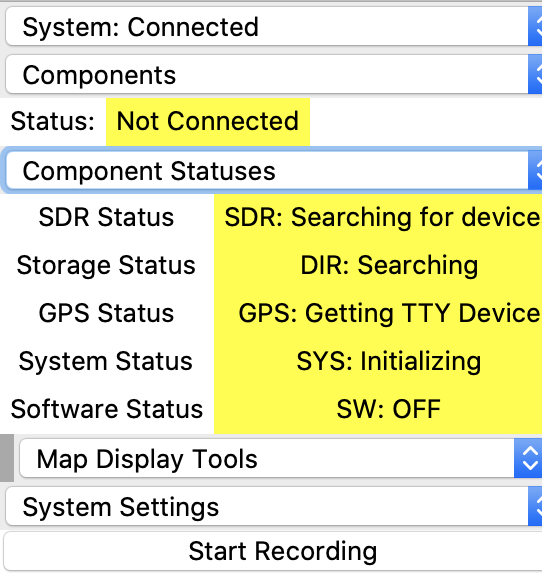
\includegraphics[scale=0.5]{ind_comp_statuses_dd.jpg}
				\label{fig:ind_comp_statuses_dd}
			\end{figure}
			\begin{enumerate}
				\item With the GCS open and connected to the payload, locate the series of drop-downs in the right-most column of the user interface.
				\item Expand the drop-down labeled "Components".
				\item Now expand the drop-down labeled "Component Statuses".
				\item Five individual component statuses will be displayed here.
			\end{enumerate}
			Here are the statuses for each of the individual components and what they mean: \\
			
			\begin{table}[htb]
			\centering
			\caption{SDR statuses and their respective meanings.}
			\begin{tabular}{||c c||}
			\hline
			State & Meaning\\ [0.5ex]
			\hline\hline
			Searching for Devices & TODO: Write explanation here. \\
			\hline
			Recycling & TODO: Write explanation here.\\
			\hline
			Initializing SDR & TODO: Write explanation here. \\
			\hline
			Ready & TODO: Write explanation here.\\
			\hline
			Failed & TODO: Write explanation here.\\ [1ex]
			\hline
			\end{tabular}
			
			\caption{Directory statuses and their respective meanings.}
			\begin{tabular}{||c c||}
			\hline
			State & Meaning\\ [0.5ex]
			\hline\hline
			Searching & TODO: Write explanation here. \\
			\hline
			Checking for Mount & TODO: Write explanation here.\\
			\hline
			Checking for Space & TODO: Write explanation here. \\
			\hline
			Recycling & TODO: Write explanation here.\\
			\hline
			Ready & TODO: Write explanation here.\\
			\hline
			Failed & TODO: Write explanation here.\\ [1ex]
			\hline
			\end{tabular}
			
			\caption{GPS statuses and their respective meanings.}
			\begin{tabular}{||c c||}
			\hline
			State & Meaning\\ [0.5ex]
			\hline\hline
			Getting TTY Device & TODO: Write explanation here. \\
			\hline
			Waiting for Message & TODO: Write explanation here.\\
			\hline
			Recycling & TODO: Write explanation here. \\
			\hline
			Ready & TODO: Write explanation here.\\
			\hline
			Failed & TODO: Write explanation here.\\ [1ex]
			\hline
			\end{tabular}
			
			\caption{System statuses and their respective meanings.}
			\begin{tabular}{||c c||}
			\hline
			State & Meaning\\ [0.5ex]
			\hline\hline
			Initializing & TODO: Write explanation here. \\
			\hline
			Ready for Start & TODO: Write explanation here.\\
			\hline
			Starting & TODO: Write explanation here. \\
			\hline
			Running & TODO: Write explanation here.\\
			\hline
			Stopping & TODO: Write explanation here.\\
			\hline
			Failed & TODO: Write explanation here.\\ [1ex]
			\hline
			\end{tabular}
			
			\caption{Software statuses and their respective meanings.}
			\begin{tabular}{||c c||}
			\hline
			State & Meaning\\ [0.5ex]
			\hline\hline
			ON & TODO: Write explanation here. \\
			\hline
			OFF & TODO: Write explanation here.\\
			\hline
			NULL & TODO: Write explanation here.\\ [1ex]
			\hline
			\end{tabular}
			
			\end{table}
\appendix		
\chapter{Reference Card}
\begin{landscape}
		\begin{multicols}{3}
		\section*{Preflight Aircraft}
			\begin{tabular*}{\columnwidth}{l @{\extracolsep{\fill}} r}
				Aircraft Docs & Check\\
				Balance & Check\\
				BATT PWR SWITCH & OFF\\
				RC/TX PWR SWITCH& OFF\\
				BATT LEVEL & Check\\
				RC/TX BATT LEVEL & Check\\
				SDR MOUNT & Secure\\
				SDR USB CONN & Secure\\
				SDR SMA CONN & Secure\\
				SDR ANT & Secure\\
				GPS & Secure\\
				GPS USB CONN & Secure\\
				PAYLOAD PWR CONN & Secure\\
				PAYLOAD USB CONN A & Secure\\
				PAYLOAD USB CONN B & Secure\\
				PAYLOAD MOUNT & Secure\\
				PAYLOAD WIFI ANT & Secure\\
				Propellers & Check\\
				Landing Gear & Check\\
			\end{tabular*}
		\section*{Pre Power On}
			\begin{tabular*}{\columnwidth}{l @{\extracolsep{\fill}} r}
				Preflight Inspection & Complete\\
				PAYLOAD SW & OFF
			\end{tabular*}
		\section*{Power On}
			\begin{tabular*}{\columnwidth}{l @{\extracolsep{\fill}} r}
				BATT PWR SW & Start\\
				SOLO LEDs & Check\\
				PAYLOAD STATUS & Check TODO\\
				RC/TX PWR SW & Start\\
				RC/TX SCREEN & Check\\
				GCS WIFI & Check\\
				GCS SOFTWARE & Start\\
				MP LINK PORT & UDP\\
				MP LINK & Connect\\
				MP Local Port & 14550\\
			\end{tabular*}
		\section*{Pre Takeoff}
			\begin{tabular*}{\columnwidth}{l @{\extracolsep{\fill}} r}
				MP HUD & Check\\
				MP PreFlight & Check\\
				GPS STATUS & Check\\
				GPS SATS & Check\\
				GPS LOCATION & Check\\
				ACFT ORIENTATION & Check\\
				AIRSPACE & CLEAR\\
				TAKEOFF Clrnce & Contact\\
			\end{tabular*}
		\section*{Payload Start Procedure}
			\begin{tabular*}{\columnwidth}{l @{\extracolsep{\fill}} r}
				PAYLOAD SW & ON\\
				PAYLOAD STATUS & Check
			\end{tabular*}
		\section*{Takeoff}
			\begin{tabular*}{\columnwidth}{l @{\extracolsep{\fill}} r}
				RC/TX FLY & Start\\
				TROTTLE & 75\%
			\end{tabular*}
		\section*{Pre Mission Start}
			\begin{tabular*}{\columnwidth}{l @{\extracolsep{\fill}} r}
				Power On & Completed\\
				MISSION & Check\\
				Wind & Check
			\end{tabular*}
		\section*{Mission Start}
			\begin{tabular*}{\columnwidth}{l @{\extracolsep{\fill}} r}
				Pre Mission Start & Completed\\
				LOCAL AIRSPACE & Clear\\
				FLIGHT MODE & AUTO
			\end{tabular*}
		\section*{Mission Stop}
			\begin{tabular*}{\columnwidth}{l @{\extracolsep{\fill}} r}
				FLIGHT MODE & AUTO
			\end{tabular*}
		\section*{Pre Landing}
			\begin{tabular*}{\columnwidth}{l @{\extracolsep{\fill}} r}
				APPROACH & CLEAR\\
				TRAFFIC & CLEAR\\
				FLIGHT MODE & LOITER
			\end{tabular*}
		\section*{Approach}
			\begin{tabular*}{\columnwidth}{l @{\extracolsep{\fill}} r}
				THROTTLE & Reduce as needed\\
				Descent Rate & $<$ 2 m/s
			\end{tabular*}
		\section*{Landing}
			\begin{tabular*}{\columnwidth}{l @{\extracolsep{\fill}} r}
				THROTTLE & Reduce as needed\\
				Descent Rate & $<$ 2 m/s\\
				THROTTLE & 0\%
			\end{tabular*}
		\section*{Payload Stop}
			\begin{tabular*}{\columnwidth}{l @{\extracolsep{\fill}} r}
				PAYLOAD SW & OFF\\
				PAYLOAD STATUS & Check
			\end{tabular*}
		\end{multicols}
\end{landscape}
\printglossaries
\end{document}
\grid
